\chapter{Nuclear Physics}

\section{Nuclear Processes}

\subsection{The Nucleus}

Rutherford's experiment consisted of a beam of $\a$-particles ($\ce{^4_2 He}$), generated by the radioactive decay of radium, directed normally onto a sheet of very thin gold foil in an evacuated chamber.

Alpha particles produce a tiny, but visible flash to light when they strike the fluorescent zinc sulphide screen, which is used as a detector, at the focus of a microscope; the screen and microscope could be swivelled around the foil to observe particles deflected at any given angle.

\begin{figure}[H]
    \centering
    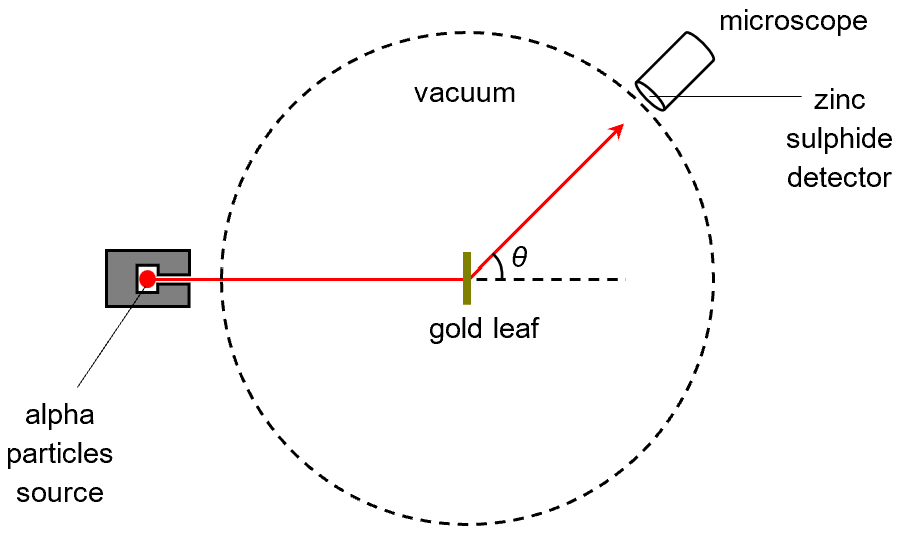
\includegraphics[scale=0.6]{media/Rutherford Alpha-Particle Scattering Experiment.png}
    \caption{The experimental set-up.\protect\footnotemark}
\end{figure}
\footnotetext{Source: \url{https://xmphysics.com/2023/01/10/18-1-1-rutherford-alpha-particle-scattering-experiment-2/}}

The following were observed:
\begin{itemize}
    \item Most of the $\a$-particles were deviated through small angles. This suggests that the atom is mostly empty space, i.e. the size of the nucleus is small compared to the atom.
    \item A small but significant percentage of the $\a$-particles were deviated through angles larger than 90$\deg$. This suggests that the mass of the atom is concentrated in the nucleus, and that the nucleus is positively charged.
\end{itemize}

These observations led to the proposal of the nuclear model of an atom, in which positively charged protons and electrically neutral neutrons are tightly packed in a very dense nucleus at the centre. A cloud of negatively charged electrons circulate around the nucleus. The nucleus provides nearly all the mass, but very little of the volume.

\begin{definition}
    Protons and neutrons in a nucleus are collective known as \vocab{nucleons}.
\end{definition}

\begin{definition}
    The \vocab{nucleon number} or \vocab{mass number} ($A$) of a nucleus is equal to the number of nucleons in it.
\end{definition}

\begin{definition}
    The \vocab{proton number} or \vocab{atomic number} ($Z$) of a nucleus is equal to the number of protons in it.
\end{definition}

Each element in the periodic table has a unique proton number.

All atoms are neutral, hence the proton number of its nucleus and the number of electrons orbiting it must be the same.

\begin{definition}
    The \vocab{unified mass constant} (u) is defined as $1/12$ of the mass of a carbon-12 atom. \[1 \text{ u} = 1.66 \times 10^{27} \text{ kg}.\]
\end{definition}

Nucleons have masses of approximately 1 u (proton mass $= 1.007$ u, neutron mass $= 1.008$ u), while electrons are much less massive (electron mass $ = 0.00055$ u).

\subsection{Nuclides and Isotopes}

\begin{definition}
    A \vocab{nuclide} is a particular type of nucleus that is specified by its proton number and neutron number.
\end{definition}

The usual notation for the representation of a nuclide is \[\ce{^A_Z X},\] where $X$ is the chemical symbol of the element, $A$ is the nucleon number and $Z$ is the proton number.

\begin{definition}
    \vocab{Isotopes} are atoms/nuclei of the same element that have the same atomic number but different mass numbers.
\end{definition}

Isotopes have the same chemical properties but different physical and nuclear properties, e.g. density, magnetic properties and radioactive tendency.

\subsection{Mass Defect and Binding Energies}

\begin{definition}
    The \vocab{mass defect} ($\D m$) of a nucleus is the difference between the observed mass $M$ of the nucleus and the total mass of the constituent nucleons.
\end{definition}

Mathematically, \[\D m = \bp{Z m_p + N m_n} - M,\] where $m_p$ is the mass of a proton, $m_n$ is the mass of a neutron, and $N = A - Z$ is the neutron number of the nuclide.

\begin{definition}
    The \vocab{nuclear binding energy} ($B$, $E_b$) of a nucleus is the energy required to completely separate the nucleons to infinity. Equivalently, it is the energy released when nucleons come together from infinity.
\end{definition}

\begin{proposition}
    The nuclear binding energy $E_b$ and mass defect of a nucleus $\D m$ is given by \[E_b = (\D m) c^2.\]
\end{proposition}

The above result is a consequence of the mass-energy equivalence due to Einstein: $E = mc^2$.

\subsection{Nuclear Reactions}

\begin{definition}
    In a \vocab{nuclear reaction}, there is a transformation of at least one element or isotope to another.
\end{definition}

A nuclear reaction must be caused by an external stimulus (e.g. the collision of nuclides).

Nuclear reactions can be represented by a nuclear equation, such as \[\ce{^{14}_7 N + ^4_2 He -> ^{17}_8 O + ^1_1 H}.\]

\begin{law}[Conservation Laws in Nuclear Reactions]
    Nuclear reactions conserve nucleon numbers, proton numbers, mass-energy and linear momentum.
\end{law}

\begin{definition}
    A nuclear reaction is said to be \vocab{exothermic} if there is a net release of energy, and \vocab{endothermic} if it requires a net energy input.
\end{definition}

The following statements about a nuclear reaction are equivalent:
\begin{itemize}
    \item The reaction is exothermic (net release of energy).
    \item The total mass of reactants is more than the total mass of the products.
    \item The total binding energy of the reactants is less than the total binding energy of the products.
\end{itemize}

Analogous equivalences are available for endothermic reactions.

\subsection{Fission and Fusion}

\begin{definition}
    The \vocab{binding energy per nucleon} is the average energy per nucleon required to completely separate the nucleons to infinity. Equivalently, it is the average energy released per nucleon when nucleons come together from infinity.
\end{definition}

The binding energy per nucleon is a measure of the stability of a nucleus. The higher the binding energy per nucleon, the more stable the nucleus is.

\begin{figure}[H]
    \centering
    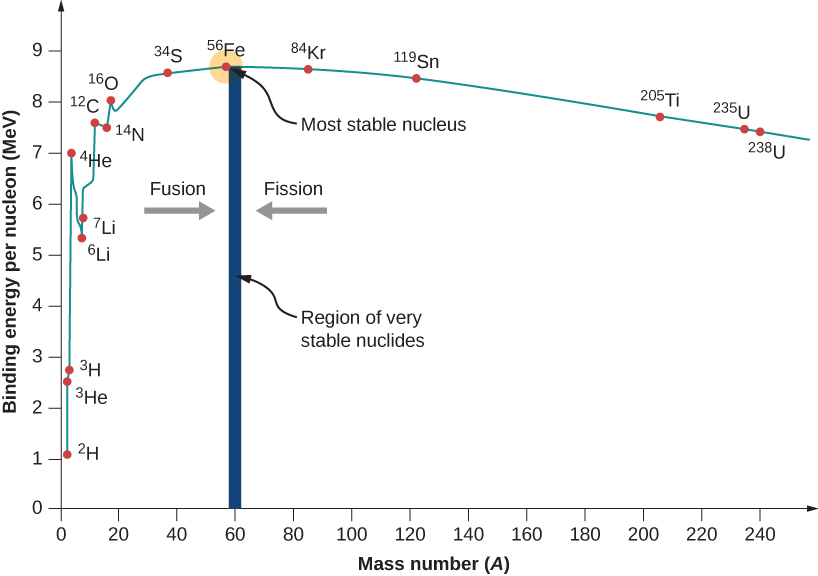
\includegraphics[scale=0.8]{media/Binding Energy Per Nucleon Variation.jpg}
    \caption{The variation of binding energy per nucleon with nucleon number.}
\end{figure}

The highest binding energy per nucleon ($\approx 8.8$ MeV) occurs at the region near $A = 56$. Observe further that the slope when $A < 56$ is very steep, while the slope when $A > 56$ is gradual.

For a nuclear reaction to release energy (exothermic), the reactants must have lower binding energy per nucleon than the products. There are two ways this can happen, namely fusion and fission.

\begin{definition}
    \vocab{Nuclear fusion} refers to two light nuclei combining to form a more massive nucleus.
\end{definition}

\begin{definition}
    \vocab{Nuclear fission} refers to the breakup of a heavy nucleus into two lighter nuclei with masses of similar orders of magnitude.
\end{definition}

Nuclear fission is typically instigated by a neutron. For instance, when a large nucleus like uranium-235 is bombarded by neutrons, one of the many fission reactions that it can undergo is the following: \[\ce{^{235}_{92} U + ^1_0 n -> ^{148}_{57} La + ^{85}_{35} Br + 3 ^1_0 n}.\] Three neutrons are produced in this reaction, which can then go on and hit other nuclei and cause a chain reaction.

Nuclear fission is ``easier'' to initiate than fusion. In fission, the uncharged neutron can be captured easily by the nuclear due to the strong nuclear force. There is no electrical interaction between the neutron and the positively charged nucleus. However, in fusion, the charged nuclei repel each other, hence they need to have a large kinetic energy before they can get close enough for the strong nuclear force to take effect. The mean kinetic energy of the nuclei is directly proportional to the absolute temperature of the gas, hence high temperatures ($\approx 10^8$ K) are required for the onset of fusion between nuclei.

\section{Radioactivity}

\subsection{Radioactive Decay}

\begin{definition}
    \vocab{Radioactive decay} is the spontaneous and random disintegration of an unstable nucleus into a more stable configuration by emitting $\a$, $\b$ and/or $\g$ radiations.
\end{definition}

Here, \emph{spontaneous} means that the decay is not affected by external or environmental factors, i.e. it cannot be sped up or slowed down by physical or chemical means. \emph{Random} means that the nucleus has a constant probability of decaying per unit time, hence the time of decay cannot be predicted.

\subsection{Count Rate}

\begin{definition}
    The \vocab{count rate} is a measure of the rate of radiation received by a radioactivity detector.
\end{definition}

For a given radioactivity level, the count rates tend to fluctuate irregularly, illustrating the random nature of radioactive decay.

\begin{definition}
    \vocab{Background radiation} is the radiation detected by a radioactivity detector when no radioactive source is nearby.
\end{definition}

Background radiation is unavoidable radiation arising from natural resources. It is roughly constant. When measuring the count rate from a source, the background count rate should be deducted from the measured count rate.

\subsection{$\a$, $\b$ and $\g$ Radiation}

\subsubsection{$\a$ Radiation}

\begin{definition}
    \vocab{$\a$-particles} contain two protons and two neutrons, i.e. a $\ce{^4_2 He}$ nucleus.
\end{definition}

The typical speed of an $\a$-particle is $0.1c$. It has low penetrating power, and is stopped by a few centimetres of air, or 0.5 mm of paper.

\begin{definition}
    \vocab{$\a$-decay} is the spontaneous decay of a nucleus with the emission of an $\a$-particle. \[\ce{^A_Z X -> ^{A-4}_{Z-2} Y + ^4_2 He}.\]
\end{definition}

Since X is unstable compared to Y, the mass of the reactant is more than the mass of the products and the decay is exothermic.

\begin{proposition}
    In $\a$-decay \[\ce{^A_Z X -> ^{A-4}_{Z-2} Y + ^4_2 He},\] let $K_\a$ and $m_\a$ be the kinetic energy and mass of the $\a$-particle respectively, and $K_Y$ and $m_Y$ the kinetic energy and mass of the daughter nucleus respectively. Then \[\frac{K_\a}{K_\a + K_Y} = \frac{m_Y}{m_\a + m_Y}.\]
\end{proposition}
\begin{proof}
    By the conservation of linear momentum, \[m_\a v_\a = m_Y v_Y \implies \frac{v_\a}{v_Y} = \frac{m_Y}{m_\a},\] where $v_\a$ and $v_Y$ are the speeds of the $a$-particle and daughter nucleus respectively. Then \[\frac{K_\a}{K_Y} = \frac{\frac12 m_\a v_\a^2}{\frac12 m_Y v_Y^2} = \frac{v_\a}{v_Y} = \frac{m_Y}{m_\a}.\] Thus, \[\frac{K_\a}{K_\a + K_Y} = \frac{\frac{K_\a}{K_Y}}{\frac{K_\a}{K_Y} + 1} = \frac{\frac{m_Y}{m_\a}}{\frac{m_Y}{m_\a} + 1} = \frac{m_Y}{m_\a + m_Y}.\]
\end{proof}

From the above result, we see that in $\a$-decay, most of the released energy ($K_\a + K_Y$) is carried by the $\a$-particle in the form of kinetic energy.

\subsubsection{$\b$ Radiation}

\begin{definition}
    \vocab{$\b$-particles} are high-speed electrons emitted from within the nucleus of an atom.
\end{definition}

The beta particles reach speeds of up to $0.9c$. It is stopped by a few metres of air, or a few millimetres of aluminimm.

\begin{definition}
    \vocab{$\b$-decay} is the spontaneous decay of a nucleus with the emission of a $\b$-particle.
\end{definition}

During $\b$-decay, a neutron changes into a proton and an electron. The new proton is retained in the nucleus, while the electron is ejected as a $\b$-particle. \[\ce{^A_Z X -> ^A_{Z+1} Y + ^0_{-1} e + \ol{\n}}.\] Here, $\ol{\n}$ represents an \vocab{antineutrino}. It has zero electric charge, and its mass is a tiny fraction of the mass of the electron.

In $\b$-decay, the total energy $Q$ released is shared, in varying proportions, between the emitted electron and the neutrino. 

\begin{figure}[H]
    \centering
    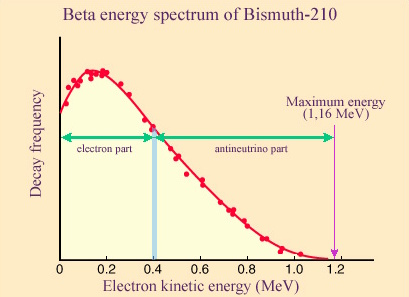
\includegraphics[scale=0.7]{media/Beta Energy Spectrum.jpg}
    \caption{The $\b$-particle energy distribution for bismuth-210.\protect\footnotemark}
\end{figure}
\footnotetext{Source: \url{https://radioactivity.eu.com/articles/phenomenon/beta_spectrum}}

\subsubsection{$\g$ Radiation}

\begin{definition}
    \vocab{$\g$-radiation} is short-wavelength electromagnetic radiation.
\end{definition}

$\g$-radiation has strong penetrating power. It is stopped by kilometre of air, or 10 cm of lead.

\begin{definition}
    \vocab{$\g$-decay} is the spontaneous decay of a nucleus with the emission of gamma radiation.
\end{definition}

Frequently, some of the energy released in $\a$- and $\b$-decay is in the form of a $\g$-ray photon. This is because $\a$- and $\b$-decay usually leave the daughter nucleus in an excited state (denoted by $^{\ast}$). The daughter nucleus emits energy in the form of a $\g$-ray photon in order to reach its ground state. \[\ce{^A_Z X^{\ast} -> ^A_Z X + \g}.\]

\subsection{Activity}

\begin{definition}
    The \vocab{activity} ($A$) of a radioactive sample is the rate at which nuclei decay, i.e. the number of disintegrations per unit time.
\end{definition}

Mathematically, \[A = -\der{N}{t},\] where $N$ is the number of undecayed particles.

The SI unit of activity is the Becquerel (Bq).

\begin{definition}
    The \vocab{decay constant} ($\l$) is the probability of decay per unit time.
\end{definition}

The SI unit of the decay constant is second$^{-1}$ (s$^{-1}$).

Activity is directly proportional to the number of undecayed particles $N$. The decay constant is the constant of proportionality between $A$ and $N$: \[A = \l N.\]

\begin{proposition}
    Given a sample of initial activity $A_0$, its activity $A$ after time $t$ is given by $A = A_0 \e^{-\l t}$.
\end{proposition}
\begin{proof}
    By definition, \[A = \l N = -\der{N}{t},\] which is a first order differential equation with solution $N = N_0 e^{-\l t}$, where $N_0$ is the original number of undecayed radioactive nuclei in the sample. Since $A = \l N$, we multiply through by $\l$ to get $A = A_0 \e^{-\l t}$.
\end{proof}

Any detector placed at a certain fixed position to measure the activity of a radioactive sample will receive a certain fraction of the radiations emitted from that sample. Thus, the received count rate $C$ ($=$ measured count rate $-$ background count rate) is directly proportional to activity $A$: \[C \propto A.\]

\begin{definition}
    The \vocab{half-life} ($t_{1/2}$) of a radioactive nuclide is the average time taken for its activity to fall to half its initial value.
\end{definition}

\begin{proposition}
    The half-life $t_{1/2}$ is related to the decay constant $\l$ by \[t_{1/2} = \frac{\ln 2}{\l}.\]
\end{proposition}
\begin{proof}
    At $t = t_{1/2}$, the activity $A = A_0/2$. Thus, \[\frac12 A_0 = A_0 \e^{-\l t_{1/2}} \implies \e^{\l t_{1/2}} = 2 \implies \l t_{1/2} = \ln 2 \implies t_{1/2} = \frac{\ln 2}{\l}.\]
\end{proof}

\begin{corollary}
    The activity $A$ after time $t$ can be written as \[A = A_0 \bp{\frac12}^{t/t_{1/2}}.\]
\end{corollary}
\begin{proof}
    We have \[A = A_0 \e^{-\bp{\frac{\ln 2}{t_{1/2}}} t} = A_0 \bp{\e^{-\ln 2}}^{t/t_{1/2}} = A_0 \bp{\frac12}^{t/t_{1/2}}.\]
\end{proof}